\documentclass{hitec}
\usepackage[UTF8]{ctex}
\usepackage{fontspec}
\usepackage[dvipsnames]{xcolor}
\usepackage{amsmath}
\usepackage{array}
\usepackage{graphicx}
\usepackage{longtable}
\usepackage{booktabs}  %用于美观表格线宽
\usepackage{multirow}  %用于跨行表
\usepackage{tabularx}  %定义表格宽度
\usepackage{float}
\usepackage{indentfirst}
\usepackage{bibentry}
%\usepackage[linkcolor=gray!40!black]{hyperref}
\usepackage[colorlinks,urlcolor=blue!50!black,linkcolor=blue!50!black,anchorcolor=blue,citecolor=blue!50!black,CJKbookmarks=True]{hyperref}
\usepackage{tcolorbox}
\usepackage{hyperref} % This line is readily ommited of it makes trouble
\tcbuselibrary{breakable,listings,skins,fitting}
\graphicspath{{figure/}}
\usepackage{newenviron}

%==========================================
% Latex 命令环境设置
%==========================================

%==========================================
% 字体设置
%==========================================
%\newfontfamily{\monoca}{Monaco}
\newfontfamily{\monoca}{Microsoft YaHei}
% \setCJKmainfont{FandolSong}
% \setmainfont{FiraSans-Light}
% \setsansfont{FiraSans-Hair}
% \setmonofont{FiraMono-Regular}

\setCJKmainfont{Microsoft YaHei}
% \setmainfont{Microsoft YaHei}
% \setsansfont{Microsoft YaHei}
% \setmonofont{Microsoft YaHei}

\setmainfont{Consolas}
\setsansfont{Consolas}
\setmonofont{Consolas}


%==========================================
% 自定义命令设置
%==========================================
\newcommand{\urllink}[2]{\href{#1}{#2}}

\newcommand{\HT}{\textsc{\raisebox{0.1em}{H}\raisebox{-0.1em}{I}%
	\raisebox{0.1em}{T}\raisebox{-0.1em}{E}\raisebox{0.1em}{C} }}

\newtheorem{thm}{定理}
\newcommand\degree{^\circ}

\newtcbox{\emphasizebox}[1][blue]{enhanced,on line,%drop fuzzy shadow,
arc=2pt,outer arc=2pt,colback=#1!5!white,colframe=#1!50!black,
boxsep=0pt,left=3pt,right=3pt,top=1pt,bottom=1pt,
colupper=blue!50!black,fit basedim=10pt,
boxrule=0.1pt,bottomrule=0.1pt,toprule=0.1pt,nobeforeafter}

%==========================================
% 自定义lsting设置
%==========================================
\newtcblisting{messagebox}{%
breakable,
left=3mm,
listing only,
boxrule=0.2mm,
colback=gray!5,
fontupper=\monoca,colupper=red!50!black,
coltext=black
}%

\newtcblisting{commandbox}{%
breakable,
left=3mm,
listing only,
boxrule=0.2mm,
colback=black,
fontupper=\monoca,colupper=red!50!black,
coltext=green
}%

\newtcblisting{codeout}{%
breakable,
left=3mm,
boxrule=0.2mm,
colback=gray!5,
fontupper=\monoca,colupper=red!50!black,
coltext=black
}%

%\lstset{
    % numbers=left,
    % %numberstyle={\color{lightgray}},
    % numberstyle={\color{green}},
    % backgroundcolor={\color[RGB]{41, 47, 51}}, %背景颜色
    % basicstyle={\color[RGB]{208, 214, 219}}, %普通字符串颜色
    % stringstyle={\color[RGB]{0, 128, 0}}, %字符串颜色
    % keywordstyle={\color[RGB]{101, 140, 230}}, %关键词颜色
    % commentstyle={\color{gray}}, %注释颜色
    % frame=none, %无边框
    % breaklines=true, %自动分行
    % language={[ANSI]C},
    % captionpos=b,
% }

\lstnewenvironment{myccode}[1][]
{\lstset{
    numbers=left,
    %numberstyle={\color{lightgray}},
    %frame=none, %无边框
    frame=lines, %上下线
    %frame=single, %边框
    language={[ANSI]C},
    breaklines=true, %自动分行
    %keywordstyle={\color{blue}}, %关键词颜色
    %stringstyle={\color{orange}}, %字符串颜色
    %stringstyle={\color{magenta}}, %字符串颜色
    %commentstyle={\color{green}}, %注释颜色
    %basicstyle={\color[black]}, %普通字符串颜色
    %captionpos=b,
    #1
        }
}
{}

%==========================================
% 标签格式
%==========================================
\hypersetup{
    colorlinks=true,
    bookmarksnumbered=true,
    pdftitle={My LaTeX2e note},
    pdfkeywords={LaTex, note},
}

%==========================================
% 摘抄格式
%==========================================
\newenvironment{literbox}
%{\begin{messagebox}
{\begin{quote}\zihao{-4}\kaishu
%{\zihao{-3}\kaishu
}
%{\end{messagebox}}
{\end{quote}}
%{}

%==========================================
% 图片路径
%==========================================
\graphicspath{{figure/}, 
{005_protocol_note/bt_picture/}, 
{009_soft_install_note/gvim_install_picture/}, 
{008_system_work_note/system_note_picture/}, 
}

%==========================================
% 水印
%==========================================
%\usepackage{draftwatermark}
%\SetWatermarkText{Zero Note} % the Text
%\SetWatermarkLightness{0.9} % the lightness from 0 to 1, default 0.8
%\SetWatermarkScale{1.0} % the scale, default 1.2


%==========================================
% 首页信息
%==========================================
\title{工作笔记}
\author{莫志烨}
\company{杰理科技}
\confidential{\textbf{-- 非限制发布 --}}

%==========================================
% 开始排版
%==========================================
\begin{document}
\begin{titlepage}
\maketitle
这是一篇关于\LaTeX 的文档,风格使用 \HT 。
\end{titlepage}

%\begin{abstract}
%本文说明如何用\LaTeX{}模板撰写报告。
%
%\end{abstract}
%提示:获取本文档的最新版本比现在开始阅读更重要。
%本文的最新版本见于:\url{https://git.coding.net/yangdawei/git.git}
\tableofcontents
\newpage
\newpage

%==========================================
% 章节内容
%==========================================
\section{\LaTeX 应用笔记}
本文档于\today 开始使用\LaTeX 作笔记文档。

\subsection{超链接应用}
超链接显示有2种:
\begin{itemize}
\item 链接和显示内容一致:\url{https://www.baidu.com}
\item 链接和显示内容不一致:\href{https://www.baidu.com}{百度链接}
\end{itemize}

\subsection{枚举项应用}
以下是枚举内容:
\begin{itemize}
\item 枚举1。
\item 枚举2。
\item 枚举3。
\item 枚举4。
\end{itemize}


\subsection{在正文中强调某个词语}
我要\emphasizebox{强abc调}这个词语。

\subsection{插入Linux命令}
\begin{commandbox}
 > sudo chsh -s zsh
\end{commandbox}

\subsection{用数字表示一个范围}
我要表示一个范围:$18\sim22$ 岁。

\subsection{插入一个Linux信息输出框}
\begin{messagebox}
On branch master
Your branch is ahead of 'origin/master' by 3 commits.
  (use "git push" to publish your local commits)
Changes not staged for commit:
  (use "git add <file>..." to update what will be committed)
  (use "git checkout -- <file>..." to discard changes in working directory)
\end{messagebox}

\subsection{测试codeout}
\begin{codeout}
codeout ccc
\end{codeout}


\subsection{基本代码块测试}
\begin{lstlisting}[language=C, numbers=left]
void main ()
{
    return;
}
\end{lstlisting}

\subsection{测试mycode}
\begin{myccode}
/* 这是一个hello工程 */
void main ()
{
    int cnt = 0;
    printf("Hello World: %d\n", cnt);
    return;
}
\end{myccode}

\subsection{空行分段 单个换行相当于空格}
老话说生活有五味,酸甜苦辣咸。苦是生命所不能避免的一味,叔本华说:“人生就是痛苦,我们可以把痛苦转换成幸福”,努力就是转化的过程,尽管在这个过程中,我们可能会感到更加辛苦。

苦,是人生的必经过程。人生就是一个“享受”痛苦和磨难的过程,这个过程是值得体会和拥有的。
人生本身就是一场与痛苦并存的旅行,并不像很多人想象的那么轻松,从生下来的那一天,我们就开始了人生的修行。

无论你生长在怎样的环
境中,你都会面临人生的各种难题。面对这些难题、困境,没有人可以不流泪流汗就轻轻松松地跨过去。经历得越多,越容易发现这个世界的真理——越怕吃苦,越有苦吃。那些心灵真正富足的人,其实都不怕吃苦。

\subsection{脚注命令}
苦\footnote{\emph 苦,是人生的必经过程。}

\subsection{引用}
\begin{quote}
老话说生活有五味,酸甜苦辣咸。
\end{quote}

\subsection{改变字体和字号}
\begin{quote}
\zihao{-5} \kaishu 老话说生活有五味,酸甜苦辣咸。
\end{quote}

\subsection{定理环境}
\begin{thm}[勾股定理]
一二三。
\end{thm}

\subsection{公式排版}
\begin{equation}
a(b+c) = ab + ac
\end{equation}

\begin{equation}
\angle ABC = \pi / 2
\end{equation}

\begin{equation}\label{eq:gougu}
AB^2 = BC^2 + AC^2
\end{equation}

\begin{equation}
90^\circ
\end{equation}

\subsection{插入图片}
%\begin{figure}[ht]
\begin{figure}[H]
\centering
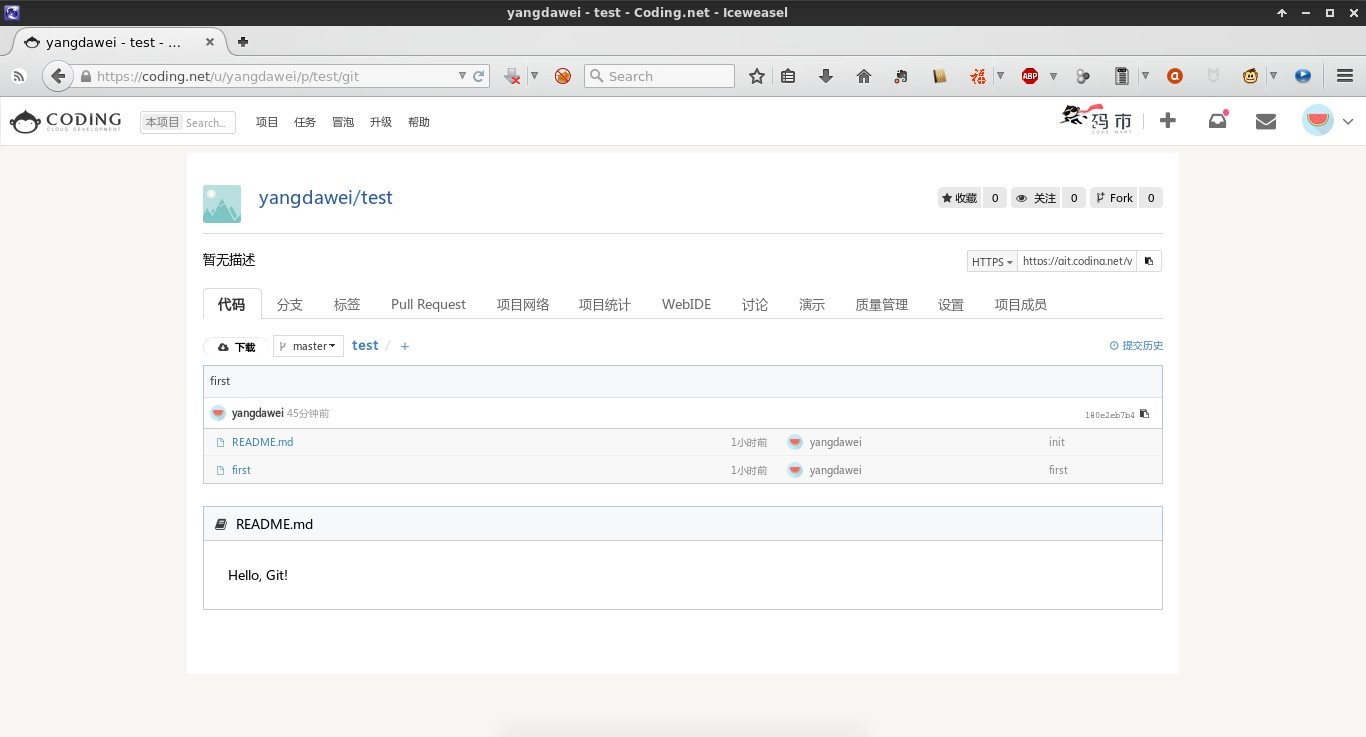
\includegraphics[height=5cm]{testcode.jpg}
\caption{建立项目}
\label{fig:createproject}
\end{figure}

\subsection{插入表格}
\begin{table}[H] %浮动环境
\begin{tabular}{|rrr|}
\hline
直角边 $a$ & 直角边 $b$ & 斜边 $c$ \\
\hline
3 & 4 & 5 \\  %分列
5 & 12 & 13 \\ %下一行
\hline
\end{tabular}
\end{table}

\subsection{引用公式和图表}
图 \ref{fig:createproject} 表示。

公式 \ref{eq:gougu} 方法。

另一种引用公式 \eqref{eq:gougu} 方法。 %添加\usepackage{amsmath}

\subsection{自定义新的命令}
使用newcommand命令。
符号度的新命令 $90\degree$ 。%注意:要加$$

\subsection{一些标点符号}
省略号\ldots \dots \# \quad \$ \quad \% \quad \& \quad \{ \quad \} \quad \_ \quad \textbackslash

中文标点使用全角输入,破折号shift+- ——,省略号shift+6……

忽略每行前面的空格,后面的空格多个当成一个,\TeX\ ing,\TeX{} ing. {\TeX} ing. 换行当空格I 
am Tex.汉字和字母自动添加空格tex。



\section{GIT学习笔记}
\subsection{合并两个提交历史}
连续在本地有两个提交, 如果需要合并这两个提交历史, 使用命令:
\begin{cmd}
 > git rebase -i HEAD~2
\end{cmd}



\section{VIM学习笔记}

\section{通信协议学习笔记}
\subsection{IIC通信协议}

\subsection{UART通信协议}

\subsection{SPI通信协议}

\subsection{IIS通信协议}
\subsubsection{IIS概述}
I2S = Inter-IC Sound = Integrated Interchip Sound = IIS,是飞利浦在1986年定义(1996年修订)的数字音频传输标准,用于数字音频数据在系统内器件之间传输,例如编解码器CODEC、DSP、数字输入/输出接口、ADC、DAC和数字滤波器等。其与IIC无关联。

\subsubsection{IIS硬件结构}
IIS是个相对来说简单的接口协议,没有地址和片选机制。在总线上,只能同时存在一个主设备和发射设备;提供时钟的设备为主设备,可以是发射设备也可以是接收设备,或者是协调两者的其他控制设备。在高端应用场合中,CODEX经常作为主设备以便精确控制IIS的数据流。

%=============================================================%
%                       插入一张图片                          %
%=============================================================%
\begin{figure}[H]
\centering
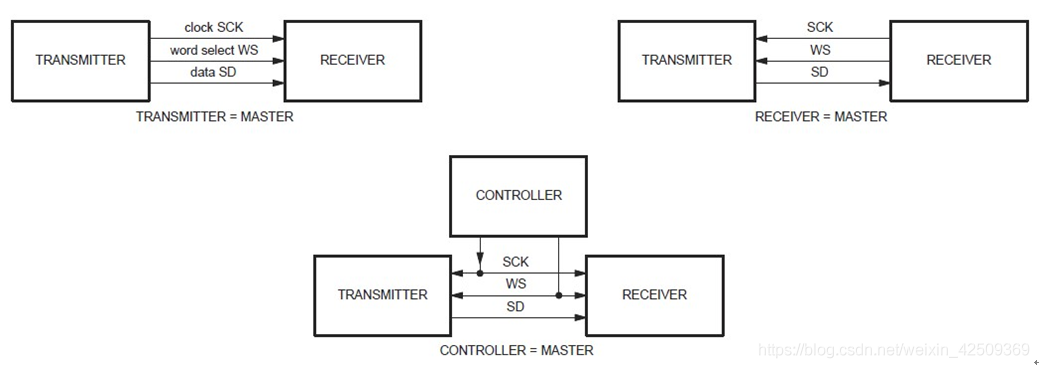
\includegraphics[scale=0.3]{iis_topo.png}
\caption{IIS硬件TOPO结构}
\end{figure}

IIS协议定义三根信号线:时钟信号SCK、数据信号SD和左右声道选择信号WS。
\begin{itemize}
\item WS:声道选择信号,表明数据发送端所选择的声道: WS=0,表示选择左声道,WS=1,表示选择右声道,同时也叫帧时钟,等于声音的采样率。
\item SCK:模块内的同步信号,从模式时由外部提供,主模式时由内部产生。
\item SD:串行数据,以二进制补码形式在数据线上传输;在WS变化后的第一个SCK脉冲,先传输最高位(MSB, Most Significant Bit)。
\end{itemize}

\subsubsection{IIS工作模式}
IIS的操作模式分为三种:标准IIS模式、左对齐模式和右对齐模式。
\begin{itemize}
\item 标准IIS模式(Phillips Standard)

IIS模式是标准左对齐格式再延迟一个时钟位变化来的,时序如下所示:
\begin{figure}[H]
\centering
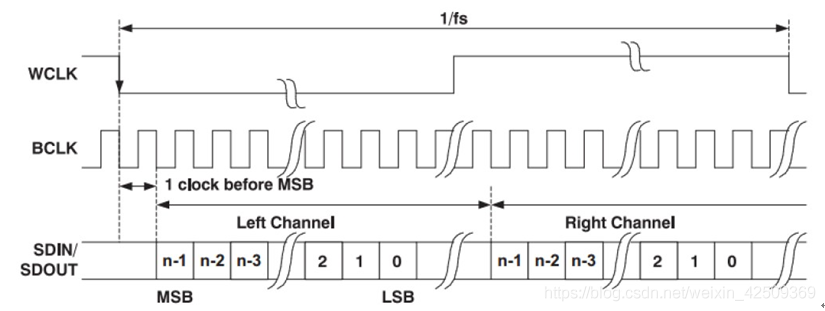
\includegraphics[scale=0.4]{iis_starndar_mode.png}
\caption{标准IIS模式}
\end{figure}
左右通道的数据MSB均是在WS变化后第二个SCK/BCLK上升沿有效。

\item 左对齐模式(Left Justified Standard)

标准左对齐格式的数据的MSB没有相对于BCLK延迟一个时钟。左对齐格式的左右声道数据的MSB在WS边沿变化后SCK/BCLK的第一个上升沿有效。具体如下图所示:
\begin{figure}[H]
\centering
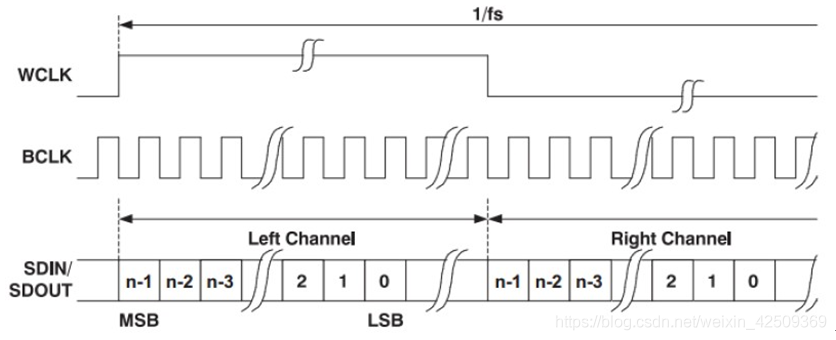
\includegraphics[scale=0.4]{iis_left_mode.png}
\caption{IIS左对齐模式}
\end{figure}
支持16~32bit字长格式;

\item 右边对齐模式(Right Justified Standard)

也叫日本格式,sony格式,具体对齐方式如下图所示:
\begin{figure}[H]
\centering
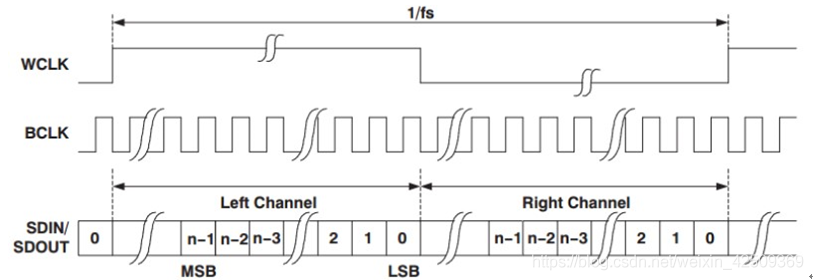
\includegraphics[scale=0.4]{iis_right_mode.png}
\caption{IIS右对齐模式}
\end{figure}
接收设备必须事先知道待传数据的字长。

\end{itemize}

\begin{messagebox}
注意左右对齐模式的WS时钟高电平为左声道,低电平为右声道,刚好与标准IIS相反。
\end{messagebox}

\subsubsection{IIS时钟频率计算}
SCK = 采样率(48K、44.1K、16K等) x  字长(16bit、24bit、32bit) x 2(左右两通道);MCLK/SCK =  384 、256 等需要参考手册说明支持哪种;

\subsubsection{一些问题解答}
\begin{itemize}
    \item \emphasizebox{384, 512fs}代表什么意思?\newline
        256fs中“fs” 就是表示audio sampling frequency, 表示在一个LR周期中BCLK的个数,比如;数据是32bit位宽,2个通道,那么fs就是32 x 2 = 64fs,可以理解为一帧有多少个sclk, fs参数结合采样率(LRCLK)可以算出BCLK,BCLK与MCLK存在分频关系,这个关系与实际通信芯片有关;
\end{itemize}

\subsection{蓝牙通信协议}
\begin{figure}[H]
\centering
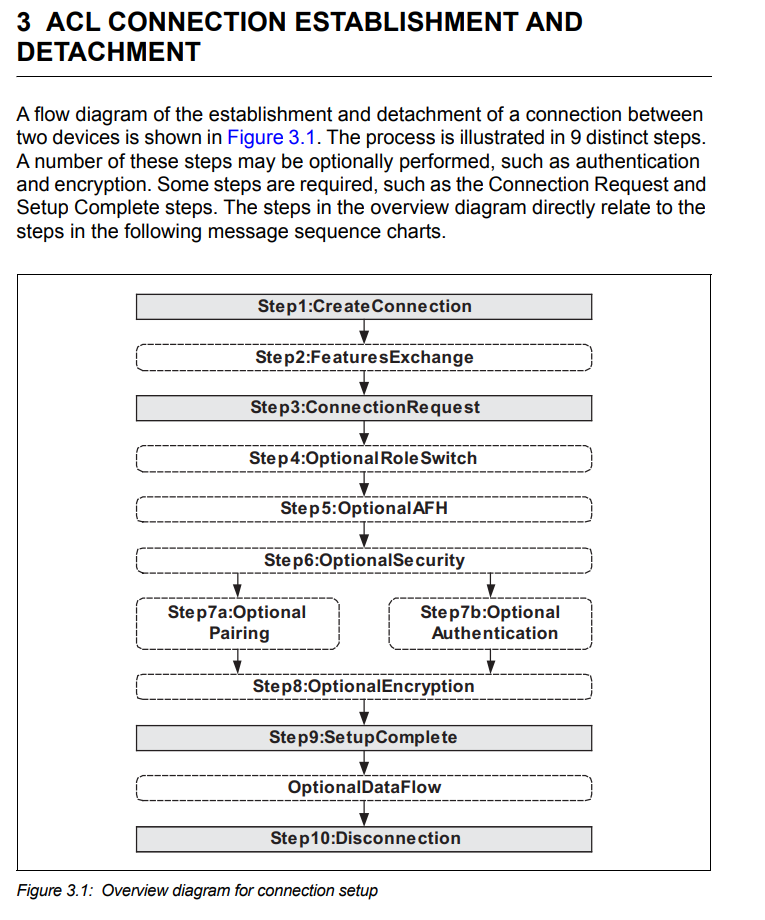
\includegraphics[height=8cm]{connection.png}
\caption{连接步骤}
\label{fig:connection}
\end{figure}

\begin{figure}[H]
\centering
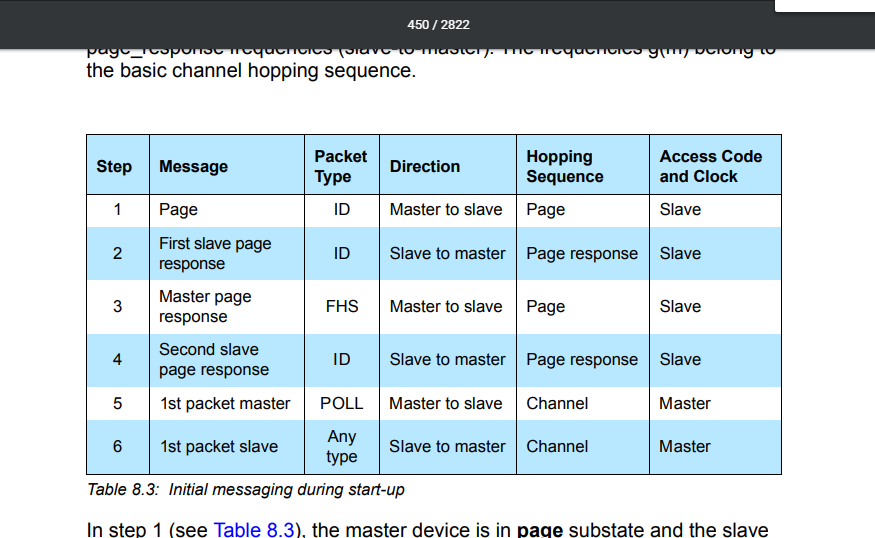
\includegraphics[height=8cm]{page_startup.png}
\caption{pagestartup}
\label{fig:pagestartup}
\end{figure}

\begin{figure}[H]
\centering
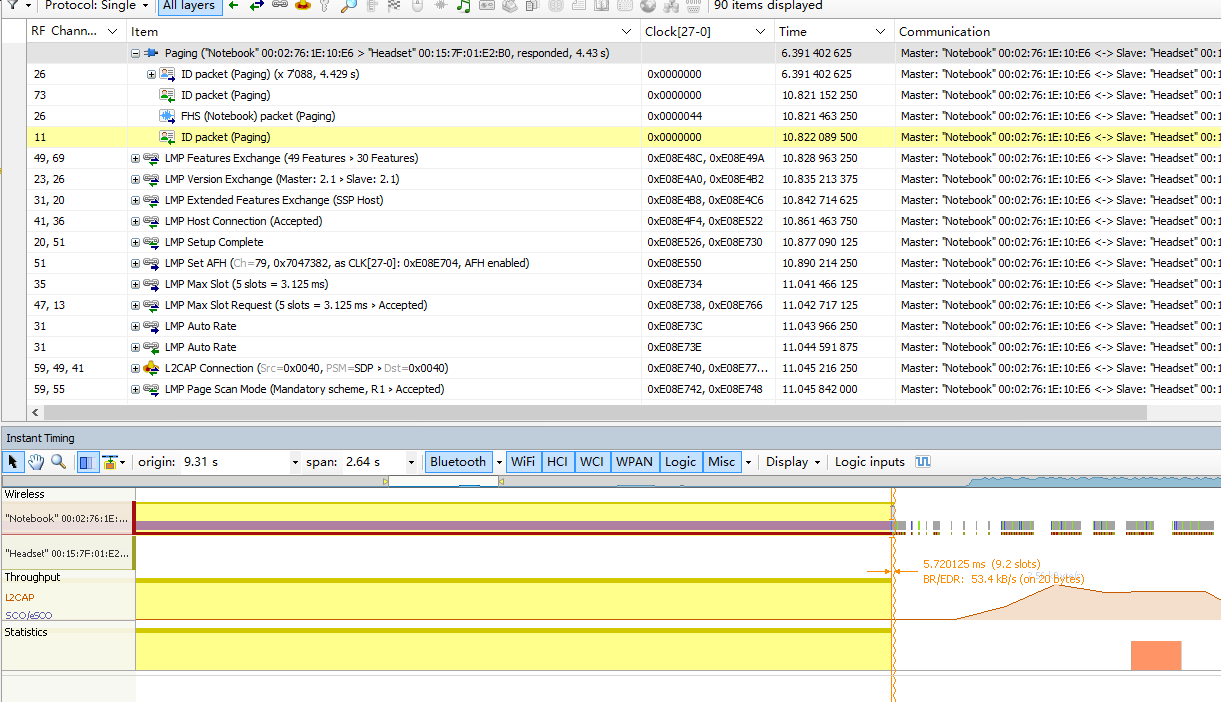
\includegraphics[height=8cm]{page_startup_data.png}
\caption{pagestartupdata}
\label{fig:page_startup_data}
\end{figure}

\href{https://en.wikipedia.org/wiki/Diffie%E2%80%93Hellman_key_exchange}{wiki链接}
\begin{figure}[H]
\centering
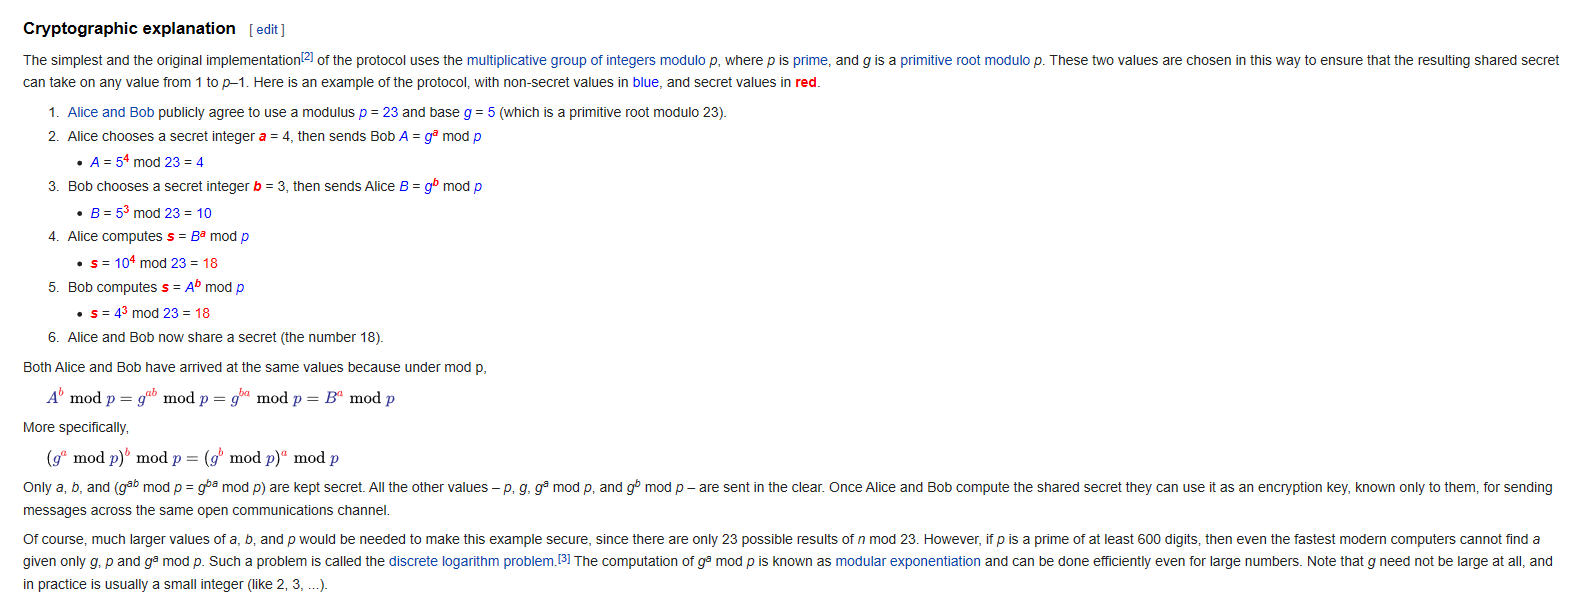
\includegraphics[height=8cm]{wiki1.png}
\caption{wiki1}
\label{fig:wiki1}
\end{figure}

\begin{figure}[H]
\centering
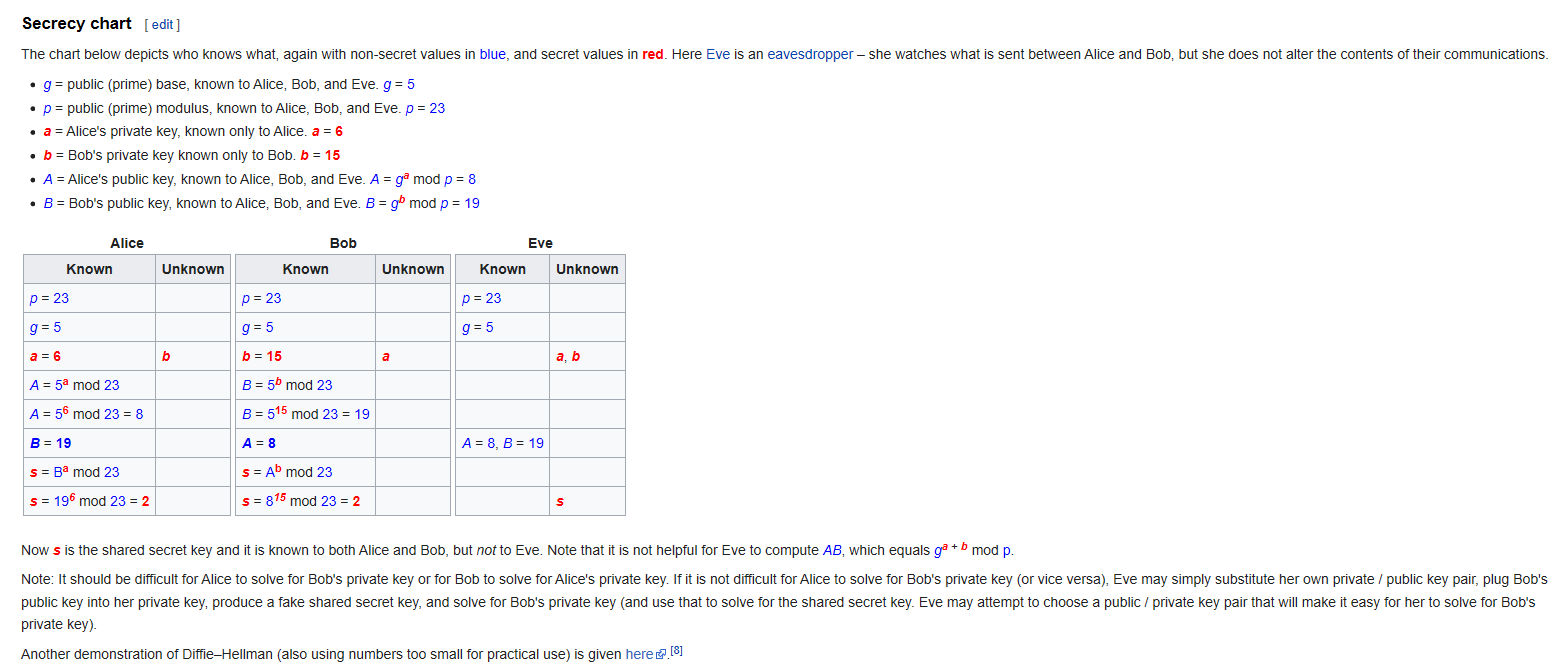
\includegraphics[height=8cm]{wiki2.png}
\caption{wiki2}
\label{fig:wiki2}
\end{figure}

\subsection{USB通信协议}



\section{文学摘抄}
%\begin{itemize}
\subsection{2020年7月28日:《破窑赋》}
%\item 2020年7月28日:《破窑赋》

%\begin{literbox}
    天有不测风云,人有旦夕祸福。蜈蚣百足,行不及蛇;雄鸡两翼,飞不过鸦。马有千里之程,无骑不能自往;人有冲天之志,非运不能自通。

    盖闻:人生在世,富贵不能淫,贫贱不能移。文章盖世,孔子厄于陈邦;武略超群,太公钓于渭水。颜渊命短,殊非凶恶之徒;盗跖年长,岂是善良之辈。尧帝明圣,却生不肖之儿;瞽叟愚顽,反生大孝之子。张良原是布衣,萧何称谓县吏。晏子身无五尺,封作齐国宰相;孔明卧居草庐,能作蜀汉军师。楚霸虽雄,败于乌江自刎;汉王虽弱,竟有万里江山。李广有射虎之威,到老无封;冯唐有乘龙之才,一生不遇。韩信未遇之时,无一日三餐,及至遇行,腰悬三齐玉印,一旦时衰,死于阴人之手。

    有先贫而后富,有老壮而少衰。满腹文章,白发竟然不中;才疏学浅,少年及第登科。深院宫娥,运退反为妓妾;风流妓女,时来配作夫人。

    青春美女,却招愚蠢之夫;俊秀郎君,反配粗丑之妇。蛟龙未遇,潜水于鱼鳖之间;君子失时,拱手于小人之下。衣服虽破,常存仪礼之容;面带忧愁,每抱怀安之量。时遭不遇,只宜安贫守份;心若不欺,必然扬眉吐气。初贫君子,天然骨骼生成;乍富小人,不脱贫寒肌体。

    天不得时,日月无光;地不得时,草木不生;水不得时,风浪不平;人不得时,利运不通。注福注禄,命里已安排定,富贵谁不欲?人若不依根基八字,岂能为卿为相?

    吾昔寓居洛阳,朝求僧餐,暮宿破窑,思衣不可遮其体,思食不可济其饥,上人憎,下人厌,人道我贱,非我不弃也。今居朝堂,官至极品,位置三公,身虽鞠躬于一人之下,而列职于千万人之上,有挞百僚之杖,有斩鄙吝之剑,思衣而有罗锦千箱,思食而有珍馐百味,出则壮士执鞭,入则佳人捧觞,上人宠,下人拥。人道我贵,非我之能也,此乃时也、运也、命也。

    嗟呼!人生在世,富贵不可尽用,贫贱不可自欺,听由天地循环,周而复始焉。
%\end{literbox}

%\end{itemize}



\end{document}


